\section{Gaussian Splatting}

\label{pre::gaussian-splatting}

Gaussian Splatting has emerged as a new approach to 3D scene representation, offering a unique blend of efficiency, flexibility, and visual quality. Unlike traditional methods that rely on explicit meshes or implicit functions, Gaussian Splatting models scenes as collections of 3D Gaussian functions. Each Gaussian is defined by its position, scale, rotation, and color, enabling efficient rendering through splatting techniques. This representation not only achieves high-quality reconstructions but also supports real-time performance, making it a powerful tool for applications ranging from interactive graphics to virtual reality.







\subsection{Core Concepts}

The fundamental idea of Gaussian splatting is the representation of a 3D scene using a set of oriented, elliptical primitives, each defined by a 3D Gaussian. These Gaussians points encode both the geometry and appearance of the scene. Mathematically, a 3D Gaussian is characterized by its mean $\boldsymbol{\mu} \in \mathbb{R}^3$ (position) and a covariance matrix $\boldsymbol{\Sigma} \in \mathbb{R}^{3 \times 3}$ (shape and orientation). The probability density function of a 3D Gaussian is given by:

\begin{equation}
f(\mathbf{x}; \boldsymbol{\mu}, \boldsymbol{\Sigma}) = \frac{1}{(2\pi)^{3/2}|\boldsymbol{\Sigma}|^{1/2}} \exp\left(-\frac{1}{2}(\mathbf{x}-\boldsymbol{\mu})^T\boldsymbol{\Sigma}^{-1}(\mathbf{x}-\boldsymbol{\mu})\right)
\label{eq:gaussian_pdf}
\end{equation}


\begin{figure}[ht]
    \centering
    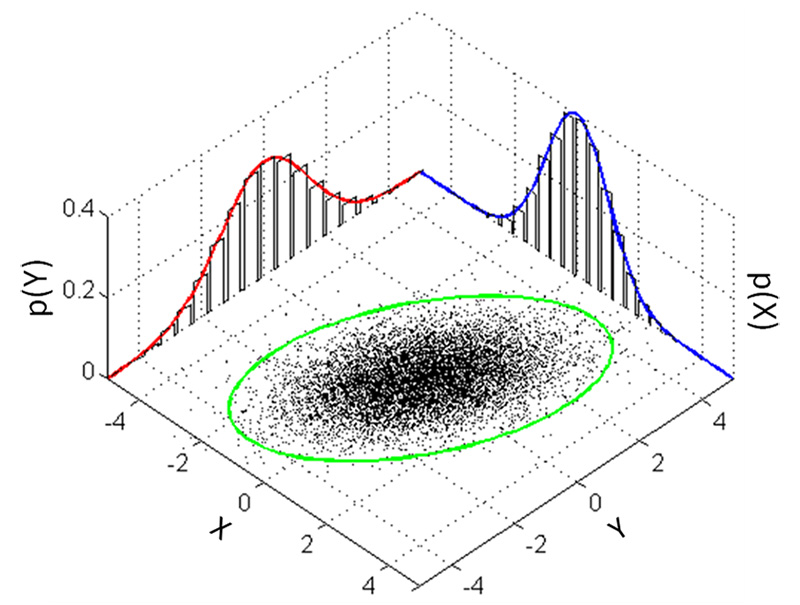
\includegraphics[width=0.5\linewidth]{assets/image2.png}
    \caption{Gaussian point represented as a projection onto a 2D surface. The ellipse corresponds to a 3D Gaussian projected onto the image plane.}
    \label{fig:gs-distribution}
\end{figure}


The function \( f \) describes how the density decreases as a point \( \mathbf{x} \) in 3D space moves away from the mean \( \boldsymbol{\mu} \), with the rate of decrease determined by the covariance matrix \( \boldsymbol{\Sigma} \). The covariance matrix \( \boldsymbol{\Sigma} \) can be decomposed using eigenvalue decomposition:

\begin{equation}
\boldsymbol{\Sigma} = \mathbf{R}\mathbf{S}\mathbf{R}^T
\end{equation}

where:
\( \mathbf{R} \) is a rotation matrix that defines the orientation of the Gaussian, and
\( \mathbf{S} \) is a diagonal scaling matrix that defines the extent (or variance) of the Gaussian along its principal axes.








\subsection{Scene Representation}

\label{pre::gs::scene-representation}

A 3D scene in Gaussian Splatting is represented as a collection of Gaussian points, each contributing to the overall geometry and appearance. Each Gaussian is defined by its mean \(\boldsymbol{\mu}\), covariance matrix \(\boldsymbol{\Sigma}\), and additional attributes such as color and opacity. Together, these Gaussians form a continuous representation of the scene, enabling high-quality rendering and efficient processing.

The representation is inherently flexible, allowing for dynamic adjustments to the scene's structure and appearance. However, this flexibility comes with a challenge: individual Gaussians do not represent meaningful objects or surfaces on their own. Instead, the collective behavior of the Gaussians defines the scene's geometry and appearance. This property, while powerful for rendering, poses significant challenges for editing, as discussed in Section \ref{pre::gs::editing}.














\subsection{Gaussian Splat Creation}

The process of creating Gaussian splats begins with an input, typically a set of images or a video. Structure-from-Motion (SfM) \citep{Snavely2006} and Multi-View Stereo (MVS) techniques are used to generate an initial sparse point cloud and camera parameters. Each point in the cloud serves as the mean \(\boldsymbol{\mu}\) of a Gaussian, while the covariance matrix and other properties are estimated from local geometry and appearance. The initial covariance matrix \(\boldsymbol{\Sigma}\) is typically set to a small isotropic value, and the optimization process refines it to better match the scene's geometry. The initial color and opacity of each Gaussian are also estimated from the input images, providing a starting point for further refinement.


The core of Gaussian splatting lies in its \textbf{differentiable optimization}. The system minimizes the difference between rendered views and input images by adjusting the Gaussian parameters. The total loss function is defined as:

\[
\mathcal{L}_{\text{total}} = \mathcal{L}_{\text{photo}} + \lambda_{\text{reg}}\mathcal{L}_{\text{reg}} + \lambda_{\text{density}}\mathcal{L}_{\text{density}}
\label{eq:loss}
\]

where \(\mathcal{L}_{\text{photo}}\) is the photometric loss (e.g., L1 or L2 loss) that compares rendered images to the input images.\(\mathcal{L}_{\text{reg}}\) is a regularization term that prevents overly large or small Gaussians, ensuring stable optimization and \(\mathcal{L}_{\text{density}}\) controls the density of Gaussians, avoiding excessive overlap or sparsity.

This optimization process adjusts the position, shape, and appearance of the Gaussians, resulting in a detailed and accurate representation of the scene. The use of gradient-based optimization ensures that the system can efficiently converge to a high-quality solution.







\subsection{Rendering Pipeline}

Rendering in Gaussian splatting involves projecting each 3D Gaussian onto the image plane. Under a perspective projection with Jacobian \(\mathbf{J}\), the covariance matrix \(\boldsymbol{\Sigma}\) of a 3D Gaussian is transformed into a 2D covariance matrix \(\boldsymbol{\Sigma}'\):

\[
\boldsymbol{\Sigma}' = \mathbf{J}\boldsymbol{\Sigma}\mathbf{J}^T
\label{eq:projection}
\]

This projected Gaussian defines an elliptical splat on the image plane. The splats are then sorted by depth and alpha-blended to produce the final image, ensuring correct occlusion and transparency effects.

The rendering pipeline is highly efficient, leveraging GPU acceleration to achieve real-time performance. By sorting the splats by depth and using alpha blending, Gaussian splatting can accurately handle complex scenes with overlapping objects and transparent materials.







\subsection{Editing}

\label{pre::gs::editing}

A significant limitation of Gaussian Splatting is its lack of editability. As described in Section \ref{pre::gs::scene-representation}, individual Gaussian points do not represent meaningful objects or surfaces on their own. Instead, the collective behavior of the Gaussians defines the scene's geometry and appearance. This makes it challenging to edit Gaussian splats directly, as changes to individual Gaussians often result in unintended artifacts or inconsistencies.

This limitation severely restricts the practical use cases of Gaussian Splatting, particularly in applications requiring manual adjustments or dynamic modifications. Addressing this challenge is a primary focus of this thesis. By developing a framework that enables intuitive and efficient editing of Gaussian splats, we aim to unlock their full potential for a wide range of applications, from animation and gaming to virtual production.









\subsection{Spherical Harmonics}
\label{pre::gs::spherical-harmonics}

To capture view-dependent effects such as specular highlights, reflections, and complex lighting interactions, Gaussian Splatting employs \textit{spherical harmonics (SH)}. Spherical harmonics provide a compact and efficient way to represent directional variations in color and lighting.

Spherical harmonics are a set of orthogonal basis functions defined on the surface of a sphere. They are commonly used in computer graphics to approximate complex lighting and material interactions. The color \(\mathbf{c}(\mathbf{v})\) of a Gaussian, as viewed from a direction \(\mathbf{v}\), is computed as a weighted sum of spherical harmonic basis functions:

\begin{equation}
\mathbf{c}(\mathbf{v}) = \sum_{l=0}^L \sum_{m=-l}^l c_{l,m} Y_{l,m}(\mathbf{v})
\label{eq:sh}
\end{equation}

Here, \(c_{l,m}\) are the spherical harmonic coefficients, which encode the directional variation of color. \(Y_{l,m}(\mathbf{v})\) are the spherical harmonic basis functions, which depend on the viewing direction \(\mathbf{v}\). \(l\) and \(m\) are the degree and order of the spherical harmonics, respectively, with \(l \geq 0\) and \(-l \leq m \leq l\).

The basis functions \(Y_{l,m}(\mathbf{v})\) are defined in spherical coordinates \((\theta, \phi)\), where \(\theta\) is the polar angle and \(\phi\) is the azimuthal angle. For example, the first few spherical harmonic basis functions are:

\begin{equation}
\begin{array}{cc}
    Y_{0,0}(\mathbf{v}) = \frac{1}{2\sqrt{\pi}}, &
    Y_{1,-1}(\mathbf{v}) = \sqrt{\frac{3}{4\pi}} \sin\theta \sin\phi, \\ \\
    Y_{1,0}(\mathbf{v}) = \sqrt{\frac{3}{4\pi}} \cos\theta, &
    Y_{1,1}(\mathbf{v}) = \sqrt{\frac{3}{4\pi}} \sin\theta \cos\phi.
\end{array}
\end{equation}

The spherical harmonic coefficients \(c_{l,m}\) are optimized during the training process. By using low-order spherical harmonics (typically up to \(L = 2\) or \(L = 3\)), Gaussian Splatting achieves a balance between quality and computational efficiency. Higher-order harmonics can capture more detailed lighting effects but require more coefficients and increase memory requirements.

